\section{Abhängigkeit der Metriken untereinander}
Die Metriken für den Kontext finden früher im Ablauf einer Anfrage an das RAG statt. Sollten diese Metriken besonders gut oder schlecht sein, lässt sich deutlich sehen, wie sich dies auf die danach folgenden Metriken auswirkt.

\begin{figure}[htbp]
    \centering
    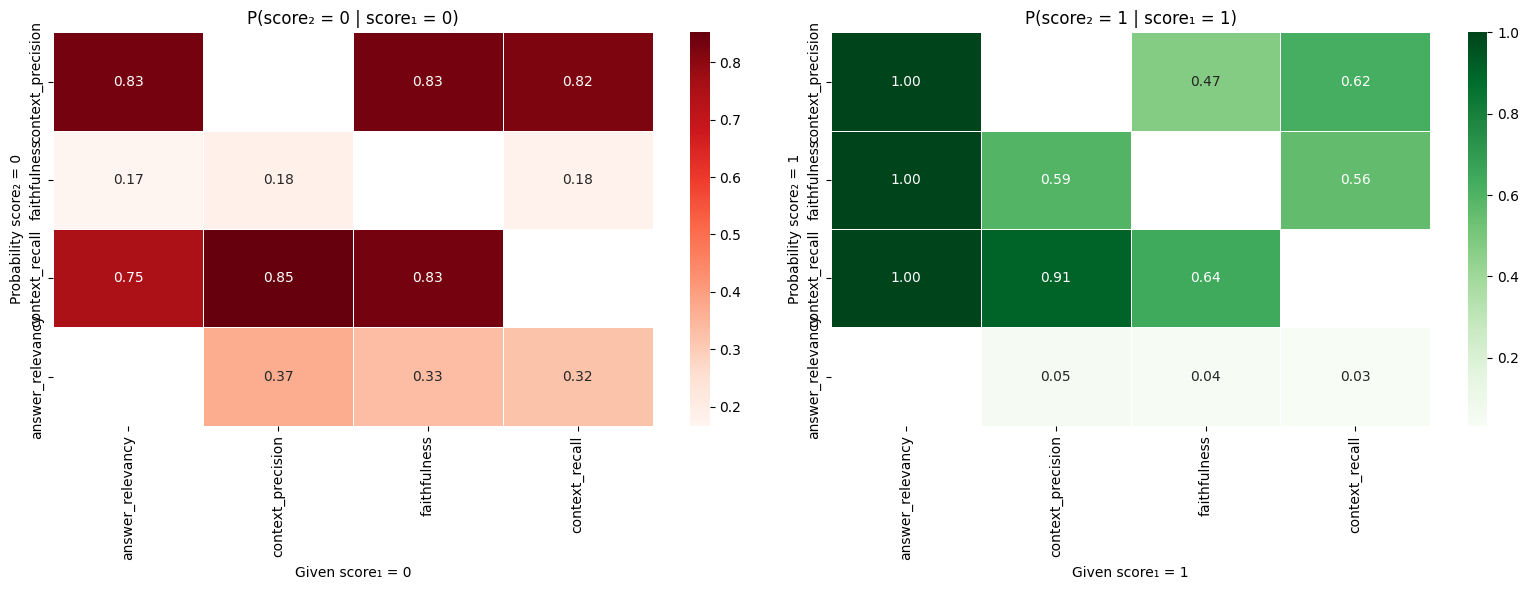
\includegraphics[width=0.8\textwidth]{images/metric_influence_400_300_O_O.png}
    \caption{Abhängigkeit der Metriken voneinander (OpenAI, 300 Fragen, 400 Dokumente)}
    \label{fig:metric_influence}
\end{figure}

Wenn die Metriken für den Kontext (context\_precision und context\_recall) eine Bewertung von 0 haben, ist die Wahrscheinlichkeit, dass die anderen Metriken auch 0 sind, relativ hoch.
In diesem konkreten Beispiel werden die Abhängigkeiten des OpenAI RAGs für die 300 Fragen gezeigt. Es lässt sich sehen, dass die faithfulness deutlich weniger von den Kontext-Metriken abhängt.

In der finalen Auswertung sollten Anwender also überlegen, Metriken wie Answer Accuracy besonders zu betrachten, wenn die Kontext-Metriken gut bewertet worden sind.